\begin{frame}{Result 2.1 - Takeaways }
    \pause
    \begin{minipage}[t]{0.45\linewidth}
    \vspace{-2.5em}
    \begin{theorem}[Reducing Exhaustion-reflection to to a Decision Procedure]
        A function $f:\Reals^n \to\Reals^m$ is exhaustion-reflecting, if we can decide for any $m$-cube $Q_m$ whether an arbitrary rational closed $n$-cube is completely contained in $f^{-1}(Q_m)$.
    \end{theorem}
    \pause
    \begin{itemize}
        \item This is very useful for proving the exhaustion-reflection property for the addition and multiplication case.
    \end{itemize}

    \end{minipage}
    \hspace{0.1em}
    \begin{minipage}[t]{0.5\linewidth}
        \pause
        \vspace{-1em}
        \color{Mahogany}
        \begin{centering}
        \textbf{Building an effective open exhaustion\\}
        \end{centering}

        % \begin{flushright}
            \only<4->{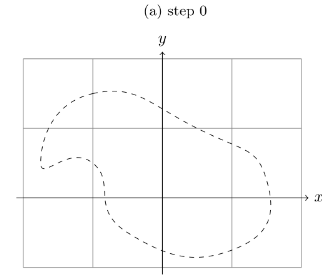
\includegraphics[width=0.48\linewidth]{tikz/step0.png}}
            \pause
            \only<5->{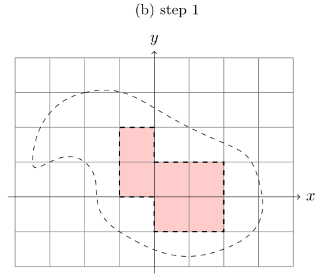
\includegraphics[width=0.48\linewidth]{tikz/step1.png} \\}
            \pause
            \only<6->{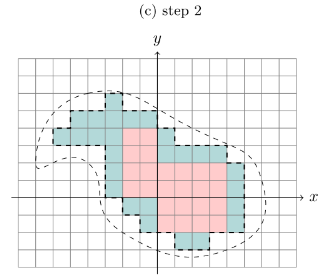
\includegraphics[width=0.48\linewidth]{tikz/step2.png}}
            \pause
            \only<7->{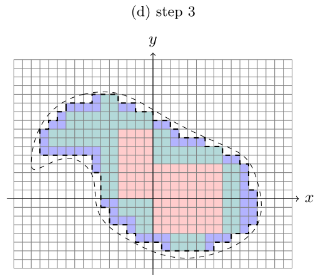
\includegraphics[width=0.48\linewidth]{tikz/step3.png}}
        % \end{flushright}
    \end{minipage}
\end{frame}